\documentclass[11pt]{article}
\usepackage[margin=1in]{geometry}
\usepackage{graphicx}
\usepackage{booktabs}
\usepackage{float}
\usepackage{amsmath}
\usepackage[hidelinks]{hyperref}
\graphicspath{{../output/figures/}}

\title{Replication Summary:\\ ``Crypto as a Marketplace for Capital Flight''\\
\large Graf von Luckner, Koepke and Sgherri (2024), IMF WP/24/133}
\author{STAT 5200, Applied Econometrics I}
\date{November 2026}

\begin{document}
\maketitle

\noindent Tables in this document are read directly from \texttt{output/tables/} by \verb|\input|, so they always match the last pipeline run. Numbers quoted in the prose come from the run of 10 November 2026 on the IMF WP-CPER export of the same day.

\section{Research question}

Can crypto exchanges serve as marketplaces where people who want foreign currency but cannot get it at the official rate buy it from people who have access to it, often through traditional capital flight channels such as trade misinvoicing? If so, the local price of bitcoin relative to its international dollar price should reveal an implied ``shadow'' exchange rate, and the gap between that rate and the official rate should measure excess demand for foreign currency and how tight capital controls are. The paper argues that crypto does not create a new channel for capital flight. Instead it monetises channels that already exist.

\section{Data}

\textbf{Paper.} Daily closing prices and volumes from CC Data for centralised exchanges, 1 January 2019 to 13 July 2023, volume weighted across exchanges. Egypt uses Binance peer to peer offers because it has no centralised exchange.

\textbf{Replication.} The IMF's public companion dataset, \emph{Crypto-based Parallel Exchange Rates} (WP-CPER, version 6.0.0). It contains the shadow rate, the official rate, the published premium and a volume series for 33 economies, and only the official rate for 31 more. I checked the IMF API as well as the Data Explorer: the dataset is \textbf{monthly only}, January 2019 to October 2025. The monthly values are period averages, which I confirmed using Ukraine's 2022 peg changes. The file has no euro area, Turkiye or Egypt series. I use the file's own shadow and official rates, and my premium, $\text{shadow}/\text{official} - 1$, matches the IMF's published premium series in all 2,095 country-months (maximum gap $5\times10^{-6}$ percentage points).

\section{Empirical strategy}

The paper is descriptive. The shadow rate is
\[
  S_t^{LCU/USD} = \frac{P_t^{BTC,LCU}}{P_t^{BTC,USD}}, \qquad \pi_t = \frac{S_t}{E_t^{\text{official}}} - 1 .
\]
\begin{itemize}
  \item \textbf{H1:} with an open financial account, arbitrage enforces the law of one price, so $\pi_t$ stays near zero.
  \item \textbf{H2:} with binding capital controls and a managed exchange rate, $\pi_t$ opens up and persists.
  \item \textbf{H3:} countries with closed financial accounts (Baba et al.\ openness index below 0.5) are the ones that ban crypto.
\end{itemize}
The paper tests H1 and H2 with country plots. I add summary statistics with Newey-West standard errors for the mean premium (lag $\lfloor 4(T/100)^{2/9}\rfloor = 3$), the share of months with $|\pi_t| > 5\%$, and $\pm 6$ month event windows around Argentina's capital controls (Decree 609/2019, 1 September 2019) and Russia's invasion of Ukraine (24 February 2022). Those two dates are my reading of the paper. The paper only says that Argentina reintroduced restrictions during the 2019 election year and that its premium rose from late 2019, and it refers to ``the Russian invasion'' for Ukraine without giving a date.

\section{Results}

\begin{figure}[H]
  \centering
  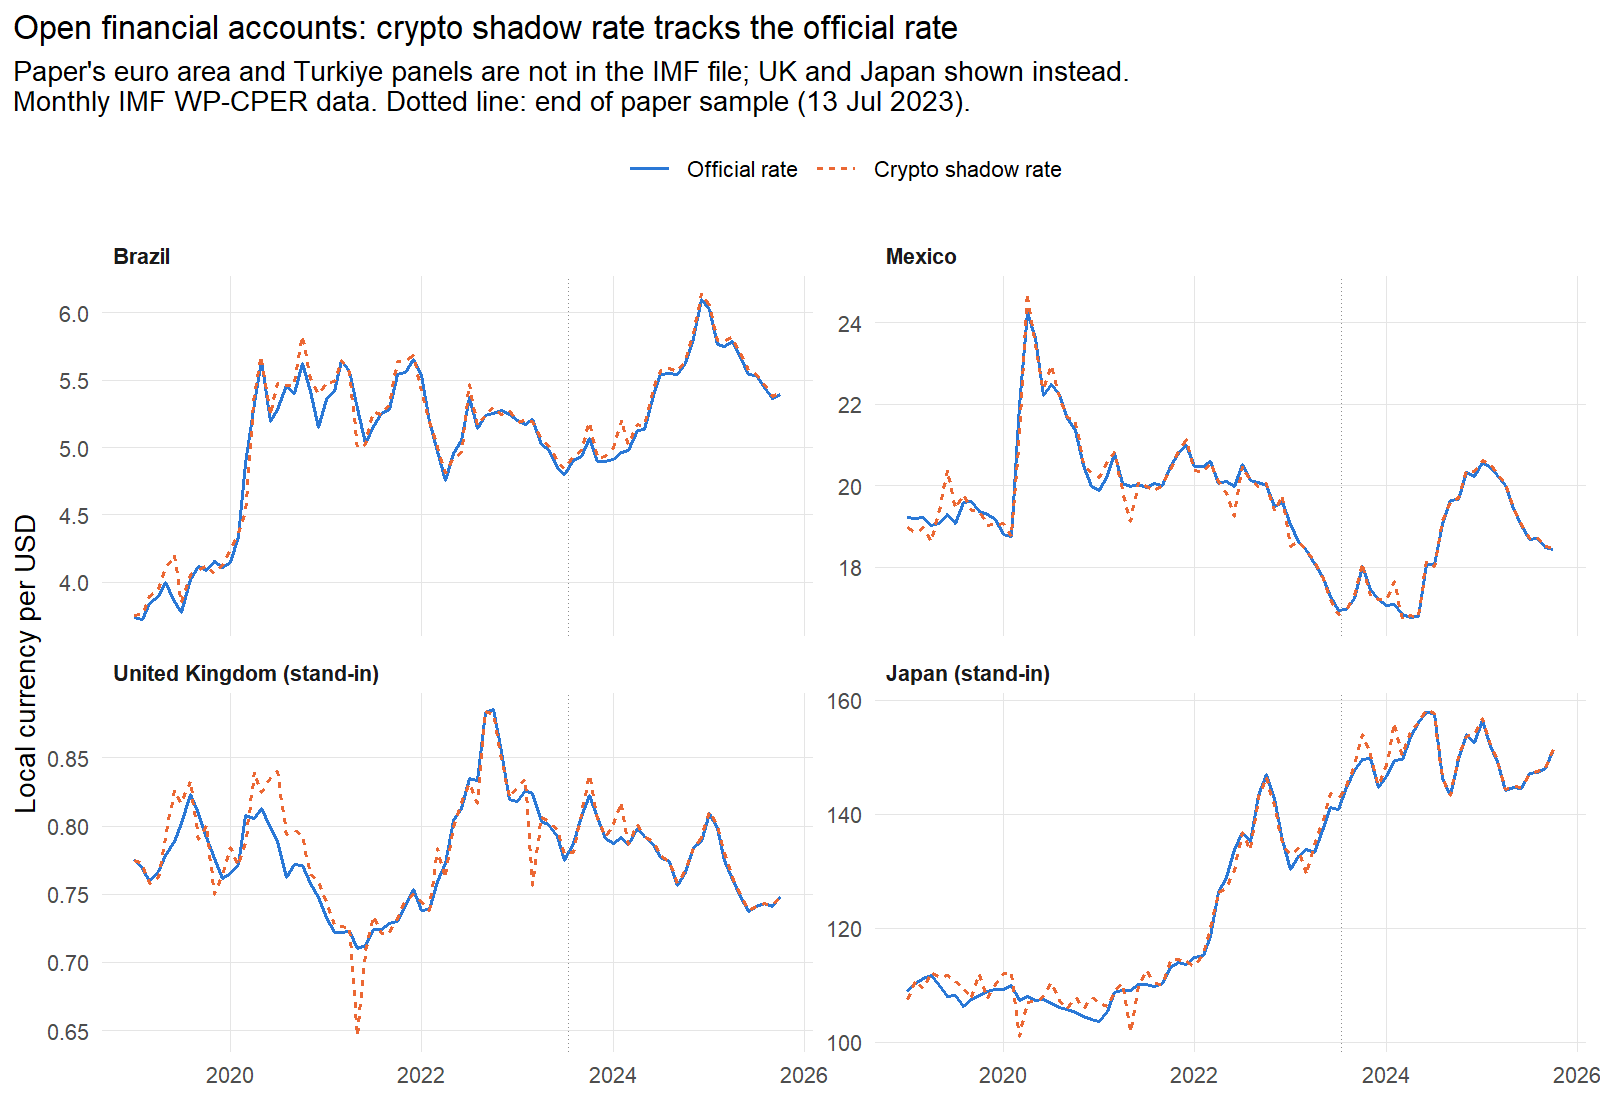
\includegraphics[width=0.85\textwidth]{fig1_open_shadow_vs_official.png}
  \caption{Open set. Brazil and Mexico as in the paper; UK and Japan stand in for the euro area.}
\end{figure}

\begin{figure}[H]
  \centering
  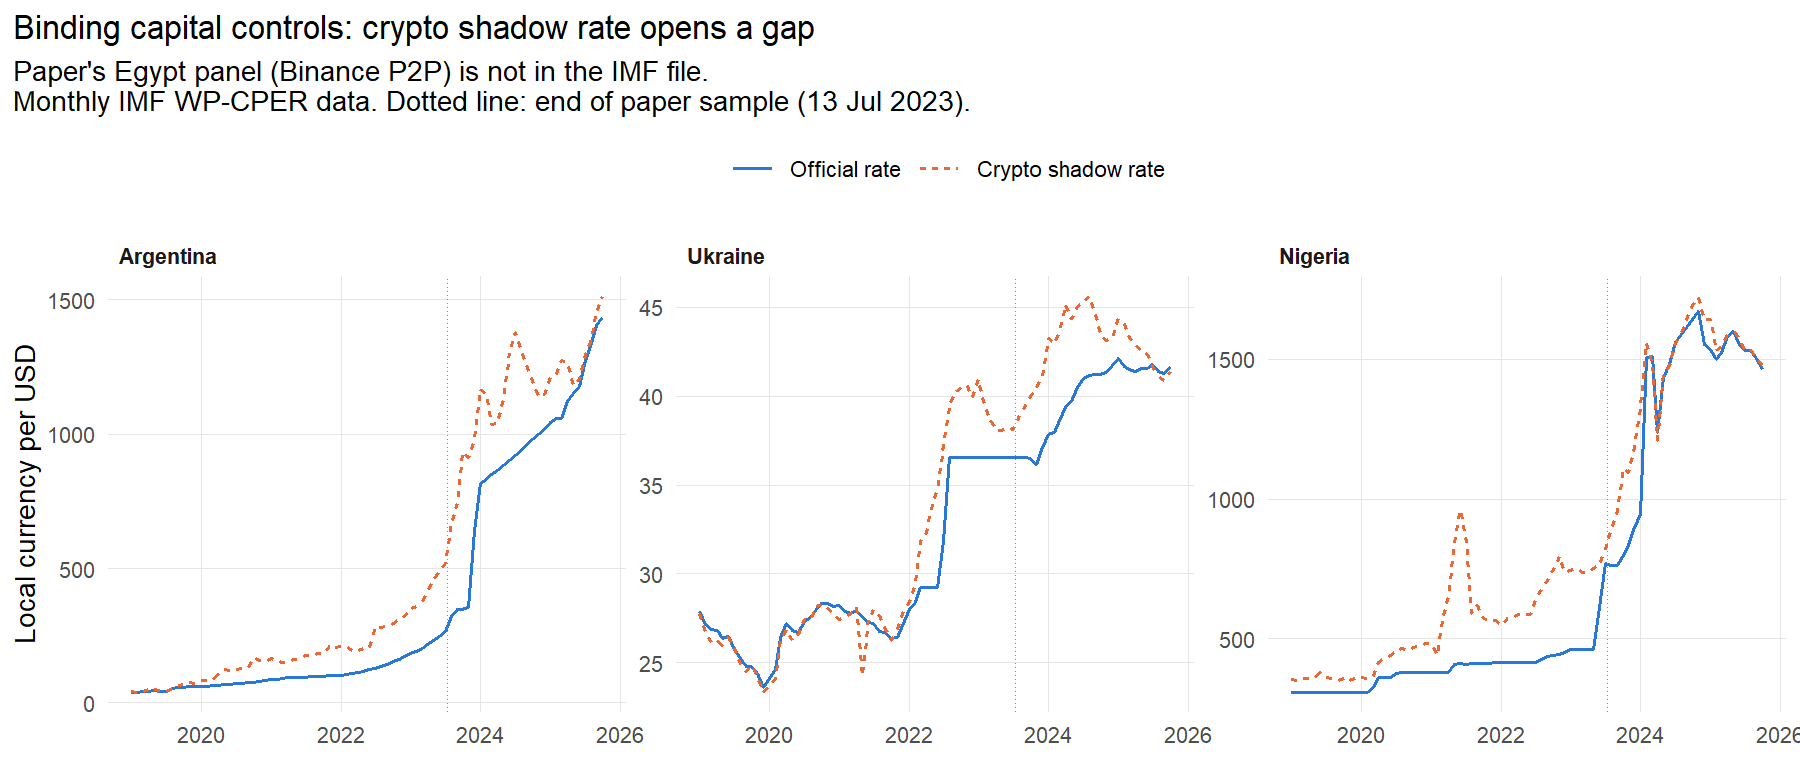
\includegraphics[width=0.95\textwidth]{fig2_controls_shadow_vs_official.png}
  \caption{Controls set. Egypt is not in the IMF file.}
\end{figure}

\begin{table}[H]
  \centering\small
  \caption{Premium summary, paper window 2019-01 to 2023-07 (monthly). Mean and NW SE in percent; ``Corr US'' is the correlation with the US premium.}
  \resizebox{\textwidth}{!}{\begin{tabular}{lrrrrrrrrr}
\hline
Country & N & Mean \% & NW SE & t & Median \% & SD & Share $>$5\% & Max \% & Corr US \\
\hline
Brazil & 55 & 0.72 & 0.34 & 2.12 & 0.74 & 2.19 & 0.05 & 8.93 & 0.83 \\
Mexico & 55 & -0.10 & 0.24 & -0.43 & -0.05 & 1.55 & 0.02 & 5.61 & 0.71 \\
United Kingdom (stand-in) & 55 & 0.41 & 0.43 & 0.97 & 0.46 & 2.56 & 0.05 & 6.53 & 0.61 \\
Japan (stand-in) & 55 & 0.39 & 0.31 & 1.29 & 0.42 & 2.03 & 0.04 & 3.91 & 0.73 \\
Argentina & 55 & 67.70 & 8.70 & 7.78 & 78.11 & 34.50 & 0.93 & 119.03 & -0.05 \\
Ukraine & 55 & 2.54 & 1.40 & 1.82 & 0.45 & 5.69 & 0.25 & 18.50 & -0.17 \\
Nigeria & 55 & 38.45 & 6.29 & 6.11 & 27.34 & 26.66 & 1.00 & 133.58 & -0.19 \\
\hline
\end{tabular}
}
\end{table}

\textbf{H1 is supported.} In the paper window, the open-set median premium is between $-0.05\%$ and $0.74\%$, and only 2 to 5\% of months exceed 5\% in absolute value. Brazil's mean of 0.72\% is statistically different from zero ($t = 2.12$) but is economically negligible. These small deviations correlate 0.61 to 0.83 with the US premium, and the US premium should be exactly zero by construction. They therefore mostly reflect noise in the international benchmark price, not local frictions.

\textbf{H2 is supported.} Argentina's median premium is 78\%, with 93\% of months above 5\%, and Nigeria's is 27\%, with every month above 5\%. Both have Newey-West $t$-statistics above 6. Ukraine's premium over the whole window is small (median 0.45\%) because it is episodic: it averaged 1.5\% in the six months before the invasion, 13.0\% in the six months after, and peaked at 18.5\% in June 2022. The paper notes that the July 2022 devaluation set the official rate near the prevailing shadow rate. In the data, the new peg of 36.57 is within 2\% of July's average shadow rate of 37.15.

\begin{figure}[H]
  \centering
  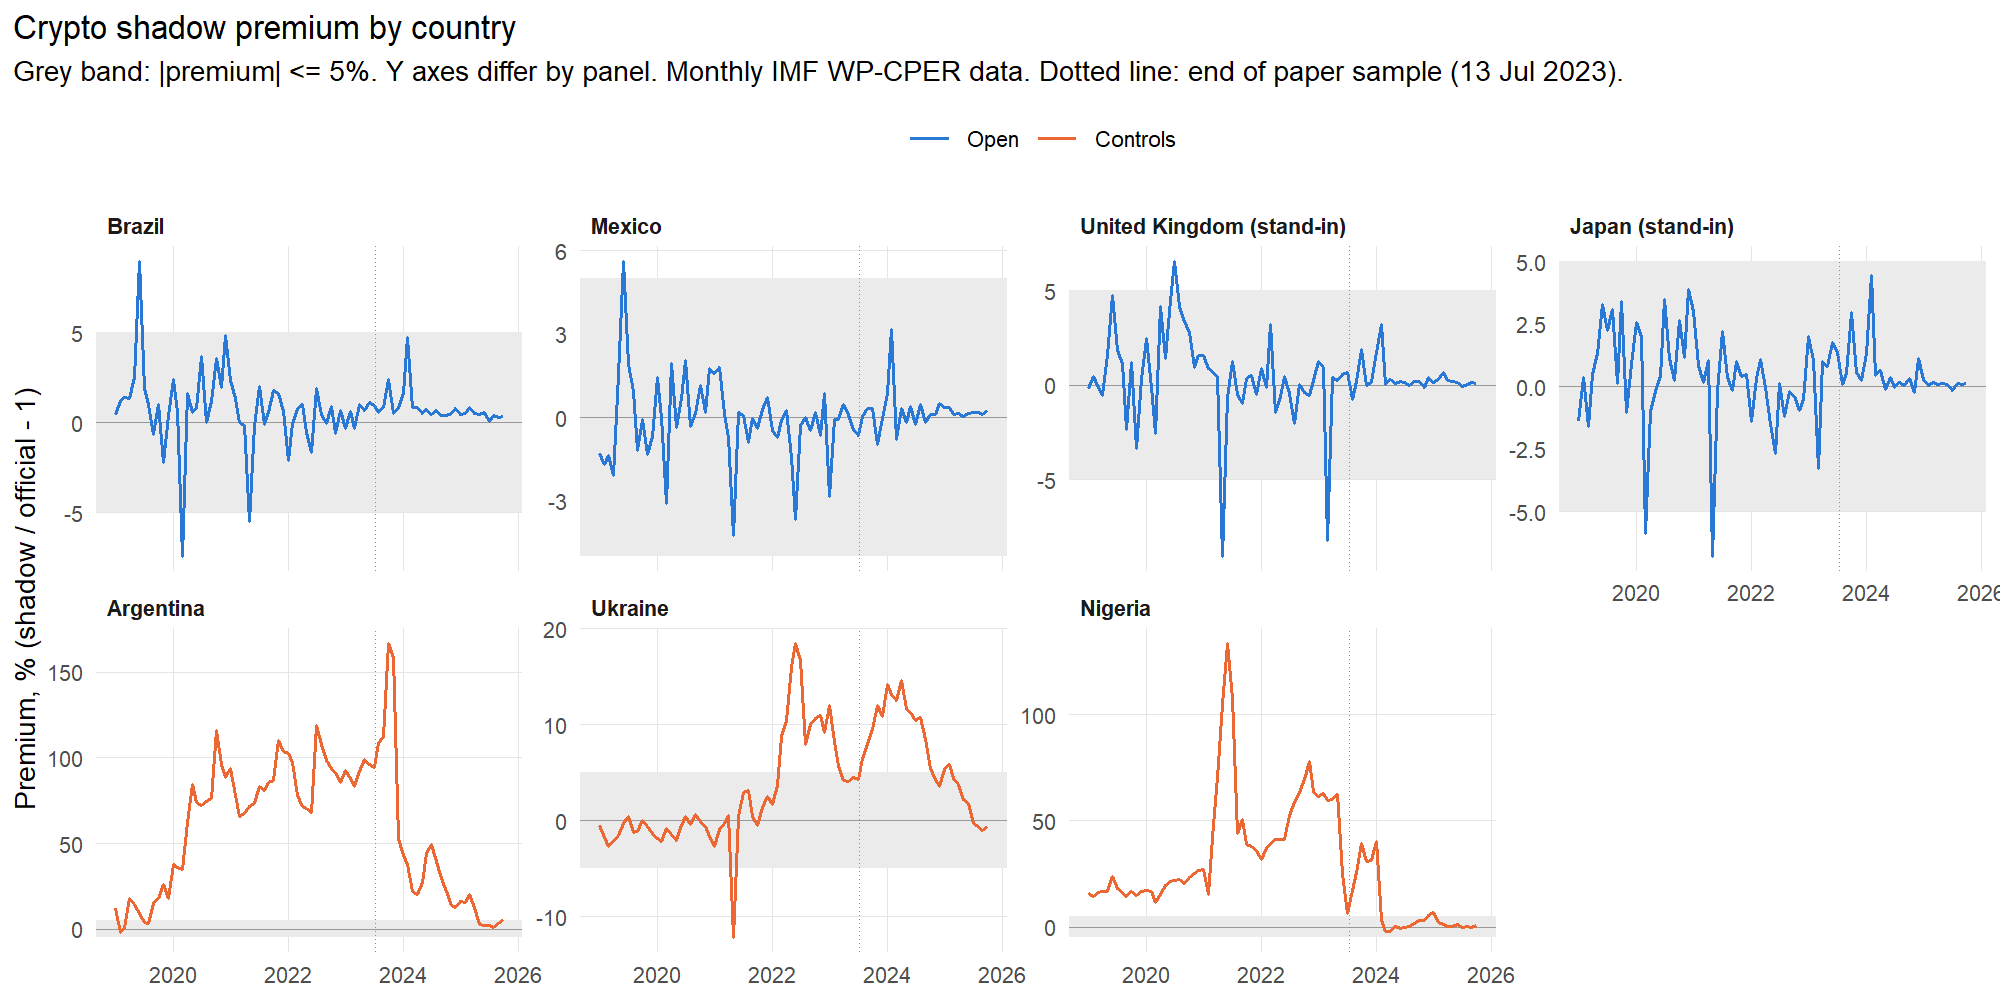
\includegraphics[width=\textwidth]{fig3_premium_panel.png}
  \caption{Premium by country with the 5\% band.}
\end{figure}

\begin{table}[H]
  \centering\small
  \caption{Event windows, $\pm 6$ months. Month 0 is excluded from pre and post means.}
  \resizebox{\textwidth}{!}{\begin{tabular}{llrrrr}
\hline
Country & Event & Pre mean \% & Month 0 \% & Post mean \% & Change pp \\
\hline
Argentina & Capital controls (Decree 609/2019) & 8.39 & 14.95 & 28.54 & 20.15 \\
Ukraine & Russian invasion & 1.48 & 3.69 & 13.04 & 11.57 \\
\hline
\end{tabular}
}
\end{table}

\begin{figure}[H]
  \centering
  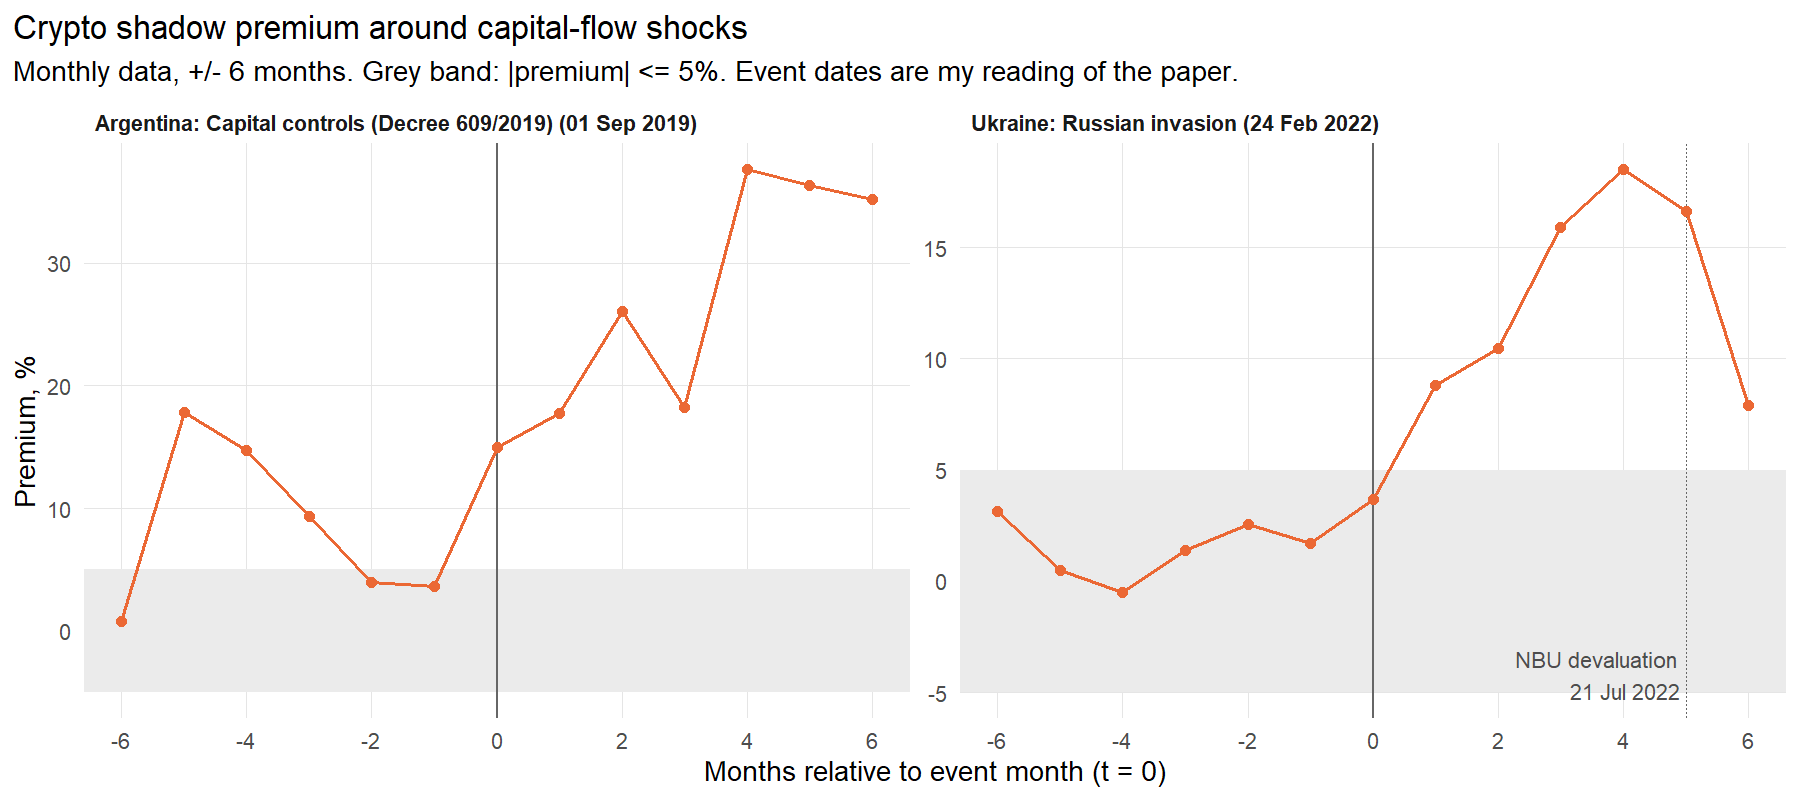
\includegraphics[width=0.95\textwidth]{fig4_event_windows.png}
  \caption{Event windows.}
\end{figure}

\textbf{Argentina is more complicated than the paper's narrative.} The premium rises from a pre-event mean of 8.4\% to a post-event mean of 28.5\% and keeps rising into 2020. However, it was already 12\% in January 2019 and 15 to 18\% in April and May 2019, before the controls. Monthly volumes in early 2019 were a fraction of their 2020 level, so this is consistent either with thin-market noise or with election-year FX pressure that started before the decree.

\textbf{H3 was not replicated.} The ban list is Library of Congress (2021) data ``updated by the authors'' and is not published, and I could not get the paper's vintage of the Baba et al.\ openness index from a reliable source. Building my own versions would be guesswork, so I skipped this hypothesis.

\section{Comparison with the paper}

\begin{tabular}{p{0.28\textwidth}p{0.66\textwidth}}
\toprule
\textbf{Matches} & Near-zero premia under open accounts (H1). Large, persistent premia in Argentina and Nigeria (H2). Ukraine's premium jumps after the invasion. The Ukraine devaluation lands close to the shadow rate. \\
\textbf{Differs} & Euro area, Turkiye and Egypt cannot be reproduced because they are not in the file. Monthly averages smooth the daily spikes, so maxima are lower and event timing is coarser. Argentina already shows a premium before September 2019. \\
\textbf{Why} & Frequency (monthly instead of daily), coverage (the IMF file has 33 crypto economies and no P2P data, so no Egypt), a possibly different exchange set and weights in version 6.0.0, and a sample that runs to October 2025 instead of July 2023. \\
\textbf{Beyond the paper} & After the paper's sample, Argentina peaks at 167\% (October 2023), falls to 53\% after the December 2023 devaluation, and stays below 5\% from May 2025, after Argentina eased FX controls for individuals in April 2025. That reversal is H2 in the other direction. Nigeria's premium disappears from February 2024 after its FX unification, while reported volumes also collapse, so a near-zero premium does not by itself mean the market works well. \\
\bottomrule
\end{tabular}

\section{Lessons learned}

\begin{enumerate}
  \item \textbf{Check what the public data actually contain before planning the replication.} The companion dataset differs from the paper's data in frequency, country coverage and sample. Three of the eight case-study countries simply are not there.
  \item \textbf{Test undocumented conventions against known events.} Whether monthly values are averages or end-of-month figures was not stated anywhere. A known peg change answered it in one line of code.
  \item \textbf{A benchmark country is essential.} The US ``premium'' should be zero by construction but moves by up to 8\%. Comparing other countries against it shows how much of an apparent deviation is just measurement noise.
  \item \textbf{Statistical significance is not the hypothesis.} With persistent series, Brazil's 0.7\% premium is significant even under HAC errors. What matters is whether the premium is large and persistent, not whether it is exactly zero.
  \item \textbf{Read the paper closely for dates.} The paper does not pin down its event dates, so any event study has to make that choice explicit.
\end{enumerate}

\section{Implications for my stablecoin premium project}

My project replaces the BTC leg with USDT: $\pi_t = P_t^{USDT,LCU}/E_t^{\text{official}} - 1$. The pipeline already isolates this step (\texttt{shadow\_rate()} and \texttt{premium()} in \texttt{code/functions.R}), so only the source of the shadow column changes. The replication suggests four design choices:
\begin{itemize}
  \item \textbf{Use daily data.} Monthly averages hide the event dynamics that matter most. I will need exchange or P2P quotes (for example Binance P2P or local centralised exchanges) at daily frequency.
  \item \textbf{Use a stablecoin leg.} USDT removes bitcoin's own price volatility and the problem of choosing an international BTC benchmark, which the US check showed is a real source of noise. Remaining noise from USDT trading slightly off its peg should be measured, for example with a US or euro area USDT premium.
  \item \textbf{Account for liquidity.} Thin markets create spurious premia, so volume or order-book depth should be a covariate or a filter.
  \item \textbf{Look at policy regimes, not just averages.} Episodes such as Nigeria in 2024 and Argentina in 2024 and 2025 show premia closing when FX regimes change. That gives natural experiments for a regression design, which the original paper does not attempt.
\end{itemize}

\appendix
\section{All economies with crypto data, paper window}
{\small \begin{tabular}{lrrrr}
\hline
Country & N & Median \% & Share $>$5\% & Max \% \\
\hline
Argentina & 55 & 78.11 & 0.93 & 119.03 \\
Nigeria & 55 & 27.34 & 1.00 & 133.58 \\
Zambia & 21 & 3.69 & 0.43 & 35.78 \\
Colombia & 50 & -3.15 & 0.20 & 9.96 \\
South Africa & 55 & 2.93 & 0.25 & 12.99 \\
India & 55 & 2.48 & 0.38 & 16.52 \\
Israel & 55 & 0.97 & 0.04 & 5.53 \\
Peru & 54 & 0.80 & 0.06 & 5.47 \\
Brazil & 55 & 0.74 & 0.05 & 8.93 \\
Chile & 54 & 0.67 & 0.04 & 6.96 \\
Vietnam & 16 & -0.61 & 0.06 & 22.13 \\
Indonesia & 55 & 0.61 & 0.02 & 9.15 \\
Philippines & 50 & 0.54 & 0.16 & 14.23 \\
Thailand & 55 & 0.50 & 0.11 & 13.65 \\
New Zealand & 55 & 0.46 & 0.09 & 9.72 \\
United Kingdom & 55 & 0.46 & 0.05 & 6.53 \\
Ukraine & 55 & 0.45 & 0.25 & 18.50 \\
Japan & 55 & 0.42 & 0.04 & 3.91 \\
Singapore & 55 & 0.41 & 0.16 & 73.24 \\
United States & 55 & 0.32 & 0.05 & 8.10 \\
United Arab Emirates & 27 & -0.24 & 0.07 & 2.73 \\
Taiwan Province of China & 17 & -0.20 & 0.00 & 2.73 \\
Malaysia & 55 & -0.19 & 0.22 & 12.43 \\
Canada & 55 & 0.18 & 0.09 & 12.20 \\
Czech Republic & 55 & 0.16 & 0.04 & 11.85 \\
Uganda & 26 & 0.08 & 0.15 & 8.60 \\
Mexico & 55 & -0.05 & 0.02 & 5.61 \\
Switzerland & 55 & 0.03 & 0.11 & 12.55 \\
Georgia & 3 & -0.03 & 0.00 & 0.69 \\
Australia & 55 & 0.01 & 0.07 & 5.88 \\
\hline
\end{tabular}
}

\end{document}
